\documentclass{beamer}
\usepackage{bm}
\usetheme{afm}

\title{Libor Market Models}
\course{Advanced Financial Modeling}
\author{\href{mailto:matteo.sani@unisi.it}{Matteo Sani}}

\begin{document}
\begin{frame}[plain]
  \maketitle
\end{frame}

\section{Libor Market Model}
\begin{frame}{Before Market Models}
  \begin{itemize}
  \item<1-> For a very long time, the market practice has been to value caps, floors and swaptions (which represent the vast majority of interest rate market) by using a formal extension of the Black (1976) model.
  \item<2-> However, this formula was applied in a completely heuristic way, under some simplifying and inexact assumptions.
    \begin{enumerate}
    \item<3-> despite the use of \emph{short rate models}; $r$ was assumed to be deterministic, so that the discounting could be factorized out of the expectation in the risk-neutral pricing formula;
    \item<4-> then, inconsistently, the forward LIBOR rates were modeled as drift-less geometric Brownian motions (hence stochastic);
    \item<5-> finally the expectation could be viewed as the price of a call option in a market with zero risk-free rate, therefore obtained through the Black’s formula.
    \end{enumerate}
  \item<6-> \textcolor{maincolor}{Unfortunately this is logically inconsistent.}
  \end{itemize}
\end{frame}

\begin{frame}{Market Models}
  \begin{itemize}
  %\item The principal idea of these approaches is to choose a different numeraire than the risk-free bank account.
    %The interest rate market is radically different from the others, e.g. commodities or equities, thus needs a own kind of modeling.
  \item<1-> There are three possible choices in interest rate modeling: \textcolor{maincolor}{short rate models} (that model one single variable), \textcolor{maincolor}{instantaneous forward rate models} (that model all infinite points of the term structure at once) and \textcolor{maincolor}{Market Models}.
  \item<2-> The latter family of (arbitrage-free) models, introduced at the end of the '90, has the following characteristics:
    \begin{itemize}
    \item<3-> models a selection of discrete real world rates (quoted in the market) spanning the term structure;
    \item<4-> chooses a different numeraire than the risk-free bank account such that these rates can be modeled log-normally;
    \item<5-> produces pricing formulas of the Black-76 type for caps/floors and swaptions;
    \item<6-> is relatively easy to calibrate to market data and can be used to price more exotic products.
    \end{itemize}
  \end{itemize}
\end{frame}
%The model we are introducing is best known generally as ”LIBOR Market Model” (LMM), or else ”Log-normal Forward LIBOR Model” or ”BraceGatarek-Musiela 1997 Model” (BGM model),

\begin{frame}{Setting the Model}
  \begin{itemize}
  \item<1-> $t = 0$ is the current time and the set $\{T_0, T_1, \dots, T_n\}$ of expiry-maturity dates is the tenor structure. %with the corresponding year fractions $\tau_i$ associated with the expiry-maturity pair $(T_{i−1}, T_i)$, for all $i > 0$;
  \item<2-> The simply-compounded forward interest rate resetting at its expiry date $T_{i-1}$ and with maturity $T_i$ is denoted by $F_i(t) = F(t; T_{i-1}, T_i)$;
  \item<3-> $\mathbb{Q}^{T_i}$ is the equivalent martingale measure (EMM) associated with the numeraire $P(\cdot, T_i)$, i.e. the $T_i$-forward measure;
  \item<4-> $\bm{W}^i$ is a $n$-dimensional \textcolor{maincolor}{correlated} Brownian motion under $\mathbb{Q}^{T_i}$, with \emph{instantaneous} correlation matrix $\bm{\rho}$, i.e. $< d\bm{W}^i(t) d\bm{W}^i(t)> = \bm{\rho} dt$.
  (\emph{Note that the superscript in a random variable refers to the measure, subscript to the component})
  \end{itemize}
\uncover<5->{
  We have already seen that $F_i$ is a martingale under the corresponding $T_i$-forward measure, on the interval $[0, T_{i-1}]$, \textcolor{maincolor}{hence each $F_i$ has a drift-less dynamics under $\mathbb{Q}^{T_i}$.}}
\end{frame}

\begin{frame}{Forward Rate Dynamics}
  \begin{block}{Proposition}
    A discrete tenor Libor Market Model assumes that the forward rates have the following dynamics under \textbf{their} associated forward measures:
    \begin{equation}
      dF_i(t) = \sigma_i(t)F_i(t)dW_i(t), t \le T_{i-1},\quad\text{ for } i = 1,\ldots, n
      \label{eq:forward_process_lmm}
    \end{equation}
    where $\sigma_i$ is assumed to be deterministic and scalar, whereas $dW_i$ is the $i$-th component of the Brownian motion.
  \end{block}
\pause
  We can show that, if $\sigma_i$ is bounded, the solution for $F_i$ is
  \begin{equation*}
    F_i(T) = F_i(t) \exp\left(\int_t^T\sigma_i(s)dW_i(s)ds - \frac{1}{2}\int_t^T
    \sigma_i^2(s)ds\right),\quad 0\le t \le T \le T_{i-1}
  \end{equation*}
\end{frame}

\begin{frame}{Exponential Martingale}
 \begin{itemize}
	\item<1-> To find the solution of the SDE $dF_t = \sigma_tF_tdW_t$ we can start with a change of variable. Let be $X_t=\ln(F_t)$ so the SDE becomes
	\begin{equation*}
	dX_t = d(\ln(F_t)) = \cfrac{dF_t}{F_t}=\sigma_tdW_t
   \end{equation*}
  \item<2-> Applying Ito's formula to $X$ we get
	\begin{equation*}
		dX_t = \cfrac{\partial X_t}{\partial t}dt + \cfrac{\partial X}{\partial F}dF + \cfrac{1}{2}\cfrac{\partial^2 X}{\partial F^2}dF^2
   \end{equation*}
	\item<3-> From the definition of $X$: $\cfrac{\partial X}{\partial t}=0$, $\cfrac{\partial X}{\partial F}=\cfrac{1}{F}$ and $\cfrac{\partial^2 X}{\partial F^2}=-\cfrac{1}{F^2}$.
\end{itemize}
\end{frame}

\begin{frame}{Exponential Martingale}
 \begin{itemize}
	\item<1-> Replacing the partial derivatives and the definition of $dF$ into the differential for $X$ and remembering that $dF^2 = \sigma_t^2 F_t^2 dt$ we get
	\only<1-1>{
	\begin{equation*}
	dX_t = \cfrac{1}{F_t}\sigma_t F_t dW_t - \cfrac{1}{2}\cfrac{1}{F_t^2}\sigma_t^2 F_t^2 dt
   \end{equation*}}
	\only<2-2>{
	\begin{equation*}
	dX_t = \cfrac{1}{\cancel{F_t}}\sigma_t \cancel{F_t} dW_t - \cfrac{1}{2}\cfrac{1}{\cancel{F_t^2}}\sigma_t^2 \cancel{F_t^2} dt
   \end{equation*}}
	\only<3->{
	\begin{equation*}
	dX_t = \sigma_t dW_t - \cfrac{1}{2}\sigma_t^2 dt
   \end{equation*}}
  \item<3-> The SDE can be solved by integrating both sides
	\begin{equation*}
	\int_0^t d(\ln(F_t)) = \ln\Big(\cfrac{F_t}{F_0}\Big)= \int_0^t \sigma_t dW_t - \cfrac{1}{2}\int_0^t\sigma_t^2 dt
	\end{equation*}
  \item<4-> And finally exponentiating
	\begin{equation*}
		F_t = F_0 \exp\Big(\int_0^t \sigma_t dW_t - \int_0^t\cfrac{1}{2}\sigma_t^2 dt\Big)
	\end{equation*}
\end{itemize}
\end{frame}

\begin{frame}{Forward Rate Dynamics in LMM}
	Now, we can ask ourselves: \emph{"what happens to Froward Rate dynamics in the other measures ?"}
 	\begin{block}{Proposition}
    Under the assumptions of the Libor Market Model, the dynamics of each $F_k$, for $k = 1,\ldots, n$, under the forward measure $\mathbb{Q}^{T_i}$ with $i \in \{1,\ldots, n\}$, is:
    \begin{equation}
      \begin{cases}
	k < i: dF_k(t) = -\sigma_k(t)F_k(t)\sum_{j=k+1}^i\cfrac{\rho_{k,j}\tau_j\sigma_j(t)F_j(t)}{1+\tau_jF_j(t)}dt + \sigma_k(t)F_k(t)dW^i_k(t) \\ \vspace{0.1cm}
	k = i : dF_k(t) = \sigma_k(t)F_k(t)dW_k^i(t) \\
	\vspace{0.1cm}
	k > i : dF_k(t) = \sigma_k(t)F_k(t)\sum_{j=k+1}^i\cfrac{\rho_{k,j}\tau_j\sigma_j(t)F_j(t)}{1+\tau_jF_j(t)}dt + \sigma_k(t)F_k(t)dW^i_k(t)
      \end{cases}
  	\label{eq:forward_rat_dynamics_lfm}
    \end{equation}
    for $t \le \min\{T_{k-1}, T_i\}$.
  \end{block}
\end{frame}

\begin{frame}{Forward Rate Dynamics in LMM (Proof)}
  \begin{itemize}
  \item<1-> By assumption, there exist a Libor Market Model satisfying \cref{eq:forward_process_lmm}.
  \item<2-> We would like to determine the deterministic functions $\mu_k^i(t, \bm{\tilde{F}}(t))$, that satisfies
    \begin{equation}
      dF_k(t) = \mu_k^i(t, \bm{\tilde{F}}(t))F_k(t)dt + \sigma_k(t)F_k(t)dW^i_k(t),\quad k\neq i
      \label{eq:forward_dynamics_in_lfm}
    \end{equation}
 where $\bm{\tilde{F}}(t)$ is the vector $(F_1(t),\ldots, F_n(t))$.
  \item<3-> Let's apply the change of measure from $\mathbb{Q}^{T_i}$ to $\mathbb{Q}^{T_k}$, then impose that the $\mathbb{Q}^{T_k}$ resulting drift is null.
  \item<4-> The Radon-Nikodym derivative of $\mathbb{Q}^{T_{i-1}}$ w.r.t. $\mathbb{Q}^{T_i}$ at time $t$ is
    \begin{equation*}
      \frac{d\mathbb{Q}^{T_{i-1}}}{d\mathbb{Q}^{T_i}}\bigg|\mathcal{F}_t = \frac{P(t, T_{i-1})P(0, T_i)}{P(0, T_{i-1})P(t, T_i)} = \zeta^i_t
    \end{equation*}
  \end{itemize}
\end{frame}

\begin{frame}{Forward Rate Dynamics in LMM (Proof)}
  	\begin{itemize}
  	\item<1-> From the forward rate definition $\cfrac{P(t,T_{i-1})}{P(t,T_i)} = 1 + \tau_i F_i$ so
    	\begin{equation*}
      	\zeta^i_t = \frac{P(0, T_i)}{P(0, T_{i-1})}(1+\tau_i F_i(t))
    	\end{equation*}
   	\item Moving to the differential, and assuming \cref{eq:forward_process_lmm} (note we are under $\mathbb{Q}^{T_i}$)
    \begin{equation*}
      \begin{aligned}
	d\zeta^i_t &= \frac{P(0, T_i)}{P(0, T_{i-1})}dF_i(t)\tau_i = \frac{P(0, T_i)}{P(0, T_{i-1})}\tau_i\sigma_i(t)F_i(t)dW^i_i(t) = \\ &= \frac{\tau_i\sigma_i(t)F_i(t)}{1+F_i(t)\tau_i}\zeta_t^idW^i_i(t)=\lambda \zeta_t^idW^i_i(t) \quad\quad \text{(we have re-introduced $\zeta$)}
      \end{aligned}
    \end{equation*}
  \item<2-> Thus, the Radon-Nikodym derivative $\zeta^i$ is an exponential martingale with associated process $\lambda$. % that is the $n$-dimensional vector $\lambda = \left(0,\ldots,\frac{\tau_i\sigma_iF_i}{1+F_i\tau_i},\ldots, 0\right)$
  \end{itemize}
\end{frame}

\begin{frame}{Forward Rate Dynamics in LMM (Proof)}
  \begin{itemize}
  \item<1-> From the Girsanov theorem:
    \begin{equation*}
      d\bm{W}^i(t) = d\bm{W}^{i-1}(t)+\bm{\rho}\lambda dt
    \end{equation*}
  \item<2-> Applying this inductively we obtain
    \begin{equation*}
  	\begin{cases}
	k < i : dW^i_j = dW^k_j + \sum\limits_{h=k+1}^i \rho^{jh}\cfrac{\tau_h\sigma_h(t)F_h(t)}{1+F_h(t)\tau_h} dt;\\
	k > i : dW^i_j = dW^k_j - \sum\limits_{h=k+1}^i \rho^{jh}\cfrac{\tau_h\sigma_h(t)F_h(t)}{1+F_h(t)\tau_h} dt;\\
  	\end{cases}
    \end{equation*}
  \end{itemize}
\end{frame}

\begin{frame}{Forward Rate Dynamics in LMM (Proof)}
	\begin{itemize}
	\item<1-> Then, inserting these into \cref{eq:forward_dynamics_in_lfm} and requiring the drift to be zero, we have:
		\begin{equation*}
			\begin{gathered}
				k < i : F_k(t)\left( \mu_k^i(t, F(t)) + \sigma_i(t)\sum_{h=k+1}^i \rho^{jh} \frac{\tau_h\sigma_h(t)F_h(t)}{1+F_h(t)\tau_h}\right) dt = 0 \\
				\implies \mu_k^i(t, F(t)) = - \sigma_i(t)\sum_{h=k+1}^i \rho^{jh} \frac{\tau_h\sigma_h(t)F_h(t)}{1+F_h(t)\tau_h}
			\end{gathered}
		\end{equation*}
		and similarly for $k > i$.
\myendproof
	\item<2-> At this point, we can turn around the argument to have the following existence result.
	\end{itemize}
\end{frame}

\subsection{Log-normal Forward Model}
\begin{frame}{Log-normal Forward Libor Model}
  \begin{block}{Proposition}
    Consider a given volatility structure $\sigma_1,\ldots, \sigma_n$, where each $\sigma_i$ is bounded, and the terminal measure $\mathbb{Q}^{T_n}$ with associated $n$-dimensional correlated Brownian motions $W^n$. If we define the processes $F_1,\ldots, F_n$ by
    \begin{equation}
      dF_i(t) = -\sigma_i(t)F_i(t)\sum_{j=i+1}^n \rho^{ij} \frac{\tau_j\sigma_j(t)F_j(t)}{1+F_j(t)\tau_j} dt + \sigma_i(t)F_i(t)dW^n_i(t)
    \end{equation}
    for $i = 1,\ldots, n$, then the $\mathbb{Q}^{T_i}$-dynamics of $F_i$ is given by \cref{eq:forward_process_lmm}, i.e. there exists a Libor Model with the given volatility structure.
  This model is often called \textcolor{maincolor}{log-normal forward Libor model} from the log-normal distribution of each forward rate under the related forward measure.
  \end{block}
\end{frame}

%Proof. First, we have to prove the existence of a solution of (2.5). For i = M
%we simply have
%dFM = σM (t)FM(t)dZM
%M (t),
%which is just an exponential martingale, where σM is bounded, thus a solution
%does exist. Now we proceed by induction: assume that (2.5) admits a solution
%for i + 1, . . . , M, then we write the i-th dynamics as
%dFi(t) = µi(t, Fi+1(t), . . . , FM(t))Fidt + σi(t)Fi(t)dZM
%i
%(t),
%where the crucial fact is that µi depends only on FK for k = i + 1, . . . , M.
%Thus, denoting F
%M
%i+1 := (Fi+1, . . . , FM)
%′
%, we can solve explicitly the above
%SDE by applying the Itˆo formula:
%d ln Fi(t) = dFi(t)
%Fi(t)
%−
%1
%2Fi(t)
%2
%σi(t)
%2Fi(t)
%2
%dt
%= µi(t, F M
%i+1(t))dt + σi(t)dZM
%i
%(t) −
%1
%2
%σi(t)
%2
%dt
%⇒ ln Fi(t) = ln Fi(0) + R t
%0
%
%µi(s, F M
%i+1(s)) −
%σi(s)
%2
%2
%
%ds +
%R t
%0
%σi(s)dZi
%i
%(s)
%⇒ Fi(t) = Fi(t) exp hR t
%0
%
%µi(s, F M
%i+1(s)) −
%σi(s)
%2
%2
%
%dsi
%exp hR t
%0
%σi(s)dZi
%i
%(s)
%i
%,
%for 0 ≤ t ≤ Ti−1 . This proves existence.
%Then, we have to prove that the process λ defined in (2.4) satisfies the
%2.1 Pricing Caps in the LMM 31
%Novikov condition (B.1), in which case the density process γ
%i
%is a Qi-martingale
%and consequently we can apply the Girsanov Theorem, retracing the same
%steps as in the proof of Proposition 2.0.2. In this regard, given an initial
%positive LIBOR term structure, as it is F(0) = (F1(0), . . . , FM(0))′
%, notice
%that all LIBOR rate processes will be always positive, thus the process λ
%in (2.4) is bounded and consequently satisfies the Novikov condition.

\begin{frame}{LFM and Black Price Equivalence}
	\begin{block}{Proposition}
		The price of the $i$-th caplet implied by the Libor market model coincides with that given by the corresponding Black caplet formula:
		\begin{equation}
			\textbf{Caplet}^{\text{LFM}}(0, T_{i-1}, T_i, K, v_i)= \tau_i P(0, T_i) Bl(K, F(0; T_{i-1}, T_i), v_i)
		\end{equation}
		where
		\begin{equation}
			v_i^2 = \frac{1}{T_{i-1}}\int_0^{T_{i-1}}\sigma_i^2(t)dt
			\label{eq:caplet_black_vol}
		\end{equation}
	\end{block}
\end{frame}

\begin{frame}{LFM and Black Price Equivalence (Proof)}
	\begin{itemize}
	%\item<1-> The discounted payoff of a cap (with unit nominal) is
	%\begin{equation*}
	%	\textbf{Cap}_{payoff} = \sum_{i=\alpha+1}^\beta \tau_iD(0, 	T_i)(F(T_{i-1}; T_{i-1}, T_i) - K)^+
	%\end{equation*}
	\item<1-> According to the risk-neutral pricing formula the price of a cap is
	\begin{equation*}
		\textbf{Cap}=\mathbb{E}^B\left[\sum_{i=\alpha+1}^\beta 	\tau_iD(0, T_i)(F(T_{i-1}; T_{i-1}, T_i) - K)^+\right]
	\end{equation*}
	\item<2-> Given the linearity of the expectation operator, we can apply the change of measure technique to move to $\mathbb{Q}^{T_i}$, i.e. the $T_i$-forward measure associated to bond price $P(\cdot,T_i)$
	\begin{equation*}
		\textbf{Cap}= \sum_{i=\alpha+1}^\beta \tau_i P(0, T_i)\mathbb{E}^{T_i}[(F(T_{i-1}; T_{i-1}, T_i) - K)^+] = \sum_{i=\alpha+1}^\beta P(0, T_i)\textbf{Caplet}
	\end{equation*}
	\end{itemize}
\end{frame}

\begin{frame}{LFM and Black Price Equivalence (Proof)}
	\begin{itemize}
	\item In order to compute
	\begin{equation*}
		\textbf{Caplet} = \mathbb{E}^{T_i}[(F_i(T_{i-1}) - K)^+]
	\end{equation*}
	just remember that under $\mathbb{Q}^{T_i}$ the process $F_i$ is a martingale.
	\item Given its log-normal distribution, the above expectation is computed as \textcolor{maincolor}{a Black and Scholes price for a stock call option whose underlying “stock” is $F_i$, struck at $K$, with maturity $T_{i-1}$, with zero constant “risk-free rate” and instantaneous percentage volatility $\sigma_i(t)$.}
\end{itemize}
\end{frame}

\subsection{Log-normal Swap Model}
\begin{frame}{A Model for Swaptions}
	\begin{itemize}
		\item<1-> The counterpart of the Log-normal Forward Libor Model among the market models, is the \textcolor{maincolor}{Log-normal Forward-Swap Model (LSM)}.
		\item<2-> It describes the evolution of the forward swap rates instead of the forward LIBOR rates, these two kind of rates being the bases of the two main markets in the interest rate derivatives world.
		\item<3-> The settings of this model are similar to the LFM, the \textcolor{maincolor}{relevant exception being the choice of a more convenient numeraire}.
	\end{itemize}
\end{frame}

\begin{frame}{Choice of the Numeraire}
	\begin{itemize}
		\item<1-> From the pricing formula of a payer swaption
		\begin{equation*}
			\textbf{PSw}=\expect{Q}\left[D(t,T_\alpha)A_{\alpha,\beta}\max(S_{\alpha,\beta}(T_\alpha)-K, 0)\right]
		\end{equation*}
		it comes clearly that the natural choice of numeraire to model the dynamics of the forward swap rate is
		\begin{equation*}
			A_{\alpha,\beta} := \sum^\beta_{i=\alpha+1}\tau_i P(t, T_i)
		\end{equation*}
		which is referred to as the \textcolor{maincolor}{annuity} or the \textcolor{maincolor}{present value of a basis point}, given $\alpha, \beta \in \{0,\ldots, n\}, \alpha < \beta$.
		\item<2-> Moreover it has the representation of the value at a time $t$ of a traded asset that is a portfolio consisting, for each $i$, of $\tau_i$ units of the zero coupon bond maturing at $T_i$, thus it is a plausible numeraire.
	\end{itemize}
\end{frame}

\begin{frame}{Choice of the Numeraire}
	\begin{itemize}
		\item<1-> Denoted by $\mathbb{Q}^{\alpha,\beta}$ the measure associated with the numeraire $A_{\alpha,\beta}$, the forward swap rate process $S_{\alpha,\beta}$ is a martingale under $\mathbb{Q}^{\alpha,\beta}$, on the interval $[t, T_\alpha]$.
		\begin{equation*}
			S_{\alpha,\beta}(t) = \cfrac{P(t,T_\alpha)-P(t,T_\beta)}{\sum_{i=\alpha+1}^{\beta}\tau_iP(t,T_i)}
		\end{equation*}
		\item<2-> The probability measure $\mathbb{Q}^{\alpha,\beta}$ is called \textcolor{maincolor}{the (forward) swap measure} related to $\alpha, \beta$.
		\item<2-> We may note that the annuity plays for the swap rate the same role as the zero coupon bond prices did for the forward rates in the LFM.
	\end{itemize}
\end{frame}

\begin{frame}{Log-normal Forward Swap Model}
	\begin{block}{Definition}
		Consider a fixed subset $\mathcal{T}$ of all the pairs of integer indices ($\alpha, \beta$) of the resettlement dates in the tenor structure $\{T_0, T_1,\ldots, T_n\}$ such that $0 \leq \alpha < \beta \leq n$ and consider for each pair a deterministic function of time $t\rightarrow \sigma_{\alpha,\beta}(t)$. A swap market model (LSM) with volatilities $\sigma_{\alpha,\beta}$ assumes that the forward swap rates have the following dynamics under their associated swap measures:
		\begin{equation}
			dS_{\alpha,\beta}(t) = \sigma_{\alpha,\beta}(t)S_{\alpha,\beta}(t)dW^{\alpha,\beta}(t),\quad t \leq T_\alpha
			\label{eq:swap_rate_dynamics}
		\end{equation}
		for $(\alpha, \beta) \in T$ pairs, where $W^{\alpha,\beta}$ is a scalar standard $\mathbb{Q}^{\alpha,\beta}$-Brownian motion.
	\end{block}
\end{frame}
%%%We can also allows for correlation between the different Brownian motions, however, this will not affect the swaption prices but only the pricing of more complicated products.
%%
%%%Remark 3. In a model with M + 1 resettlement dates it is possible to model
%%%only M swap rates as independent. The two typical choices of possible T
%%%pairs
%%%identify the following substructures:
%%%• the regular SMM, which models the swap rates S0,M, S1,M, . . . , SM−1,M,
%%%i.e.
%%%T
%%%pairs = {(0, M),(1, M), . . . ,(M − 1, M)} ;
%%%• the reverse SMM, which models the swap rates S0,1, S0,2, . . . , S0,M, i.e.
%%%T
%%%pairs = {(0, 1),(0, 2), . . .,(0, M)} .

\begin{frame}{LSM and Black Price Equivalence}
	\begin{block}{Proposition}
		The price of a payer swaption implied by the swap market model coincides with that given by the corresponding Black swaptions formula:
		\begin{equation}
			\textbf{PSw}^{LSM}(T_\alpha,T_\beta,K,v_{\alpha,\beta})=
			A_{\alpha, \beta}(0) \textbf{Sw}^{Bl}(K,S_{\alpha,\beta}, v_{\alpha,\beta})
			\label{eq:black_swaptions}
		\end{equation}
		where
		\begin{equation*}
			\begin{gathered}
				v_{\alpha,\beta}^2(T) =\frac{1}{T_\alpha}\int_0^T\sigma_{\alpha,\beta}(t)^2dt
			\end{gathered}
		\end{equation*}
	\end{block}
\end{frame}

\begin{frame}{LSM and Black Price Equivalence (Proof)}
	\begin{itemize}
		\item From the risk-neutral pricing formula after the change of numeraire (to the annuity)
		\begin{equation*}
			\begin{aligned}
				\textbf{Sw}&=\mathbb{E}^B\left[D(0,T_\alpha)A_{\alpha,\beta}(T_\alpha)(S_{\alpha,\beta}(T_\alpha)-K)^+\right] = \\
				&=\mathbb{E}^{\alpha,\beta}\left[\frac{A_{\alpha,\beta}(0)}{A_{\alpha,\beta}(T_\alpha)}A_{\alpha,\beta}(T_\alpha)(S_{\alpha,\beta}(T_\alpha)-K)^+\right] = \\
				&= A_{\alpha,\beta}(0)\mathbb{E}^{\alpha,\beta}\left[(S_{\alpha,\beta}(T_\alpha)-K)^+\right]
			\end{aligned}
		\end{equation*}
		\item Given the swap rate log-normal distribution of \cref{eq:swap_rate_dynamics}, computing the last expectation leads to Black’s formula for swaptions.
		\item Indeed, the above expectation is \textcolor{maincolor}{the classical Black and Scholes price for a call option whose underlying “asset” is $S_{\alpha,\beta}$, struck at $K$, with maturity $T_\alpha$, with 0 constant “risk-free rate” and instantaneous percentage volatility $\sigma_{\alpha,\beta}(t)$.}
	\end{itemize}
\end{frame}

\subsection{Incompatibility between LFM and LSM}
\begin{frame}{Incompatibility between LFM and LSM}
	A crucial question rises: \textcolor{maincolor}{are the two main Market Models, theoretically consistent ?}
	Can the assumptions of log-normality of both LIBOR forward rates and forward swap rates coexist?
	\pause

	In order to give an answer we can proceed as follows:
	\begin{enumerate}
		\item<2-> assume the hypothesis of the LFM, namely that each forward rate $F_i$ is log-normal under its related forward measure $\mathbb{Q}^i$;
		\item<3-> apply the change of measure to obtain their dynamics under the swap measure $\mathbb{Q}^{\alpha,\beta}$, for a choice of $(\alpha,\beta) \in T$ pairs;
		\item<4-> apply the It$\hat{o}$’s formula to obtain the resulting dynamics for the swap rate $S_{\alpha,\beta}$ under $\mathbb{Q}^{\alpha,\beta}$;
		\item<5-> check if this distribution is log-normal, as it is under the hypothesis of the LSM.
	\end{enumerate}
	\uncover<6->{
		\textcolor{maincolor}{Unfortunately, the answer is negative}.}
\end{frame}

\begin{frame}{Incompatibility between LFM and LSM}
	\begin{itemize}
		\item<1-> However, from a practical point of view, this incompatibility seems to weaken considerably.
		\item<2-> Indeed, simulating a large number of realizations of $S_{\alpha,\beta}(T_\alpha)$ with the dynamics induced by the LFM one can compute its numerical density and compare it with the log-normal density.
		\begin{center}
			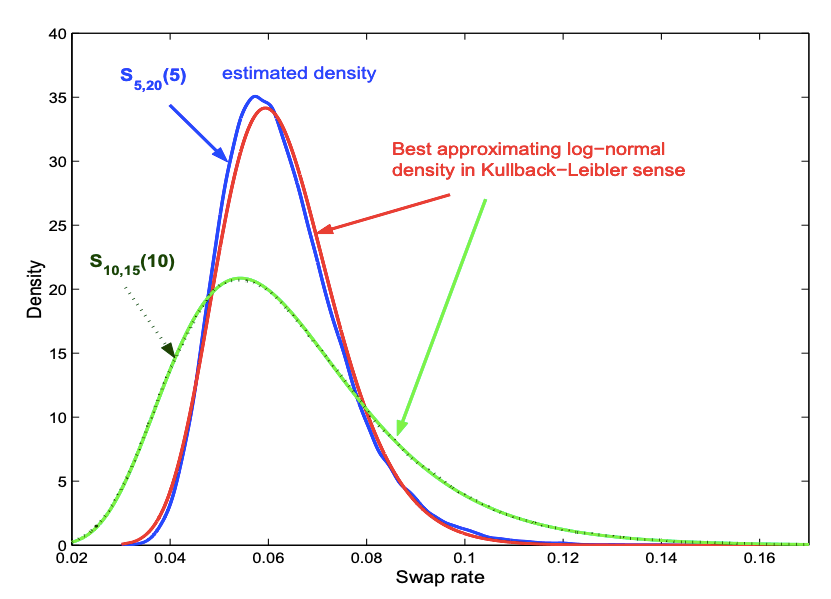
\includegraphics[width=0.45\linewidth]{images/swap_rate_LFM}
		\end{center}
	\end{itemize}
\end{frame}

\begin{frame}{Incompatibility between LFM and LSM}
	\begin{itemize}
		\item<1-> Consequently, it has been argued that, in normal market conditions, the two distributions are hardly distinguishable.
		\item<2-> Once ascertained the mathematical inconsistency of these two models, we must admit that the LSM is particularly convenient when pricing a swaption, because it yields the practice Black’s formula for swaptions. However, for different products, even those involving the swap rate, there is no analytical formula in general.
		\item<3-> The problem left is choosing either of the two models for the whole market. After that choice, the half market consistent with the model is calibrated almost automatically, thanks to Black’s formulas, but the remaining half is more intricate to calibrate.
	\end{itemize}
\end{frame}

\begin{frame}{Proposed Solution}
	\begin{itemize}
		\item<1-> \textcolor{maincolor}{Since the LIBOR forward rates, rather than swap rates, are more natural and representative coordinates of the yield curve usually considered}, besides being mathematically more manageable, the better choice of modeling may be to \textcolor{maincolor}{assume as framework the Log-normal Forward Libor Model}.
		\item<2-> Thus, hereafter, we are working under the hypothesis of the LFM.
		\item<3-> If we choose one of the discount bonds $P(\cdot, T_i)$ as a numeraire, one forward rate will be a martingale, however, the swap rate being a combination of several forward rates, will not.
		\item<4-> We thus conclude that \textcolor{maincolor}{swaption pricing via Black’s formula is not possible in the LFM}.
	\end{itemize}
\end{frame}

\begin{frame}{Proposed Solution}
	\begin{itemize}
		\item<1-> Brigo and Mercurio derived a complex expression for the swap rate dynamics under the $T$-forward measure induced by the numeraire $P(\cdot, T_i)$.
		\item<2-> But it is not much manageable. There exist, however, very good approximate formulas to the swaption volatility which can be directly used to calibrate to a matrix of quoted swaption volatilities.
		\item<3-> Also, \textcolor{maincolor}{performing a Monte Carlo simulation to obtain the swaption price is anyway feasible.}

		%\item The LFM, unfortunately, does not feature a known distribution for the joint dynamics of forward rates: to evaluate swaptions, \textcolor{maincolor}{we have to resort to Monte Carlo simulation.}
	\end{itemize}
\end{frame}

\section{Monte Carlo Pricing}

\begin{frame}{Monte Carlo Pricing of Swaptions (LFM)}
	\begin{itemize}
		\item While Black-76 prices individual caplets/swaptions in isolation, the LFM models the \textbf{joint dynamics} of the entire forward curve.
		\item<2-> In order to simulate all the processes involved in the payoff, their joint dynamics (SDEs) is discretized numerically, e.g. with the Euler scheme.
		\item It is the standard for path-dependent interest rate derivatives because it is calibrated directly to market-quoted volatilities.
		\item Rates $F_i(t)$ are modeled as diffusion processes. Because a swaption depends on a basket of these rates, we cannot price them independently; we must simulate the whole vector of rates simultaneously.
	\end{itemize}
\end{frame}

\begin{frame}{Monte Carlo Pricing of Swaptions (LFM)}
	\begin{itemize}
		\item Recall the price of a payer swaption:
		\begin{equation*}
			\begin{aligned}
				\textbf{PSw} = \expect{Q}&\left[D(0, T_\alpha) (S_{\alpha,\beta}(T_\alpha) - K)^+ \sum_{i=\alpha+1}^\beta \tau_i P(T_\alpha, T_i)\right] \\
				&= P(0, T_i)\mathbb{E}^\alpha\left[(S_{\alpha, \beta}(T_i) - K)^+ \sum^\beta_{i=\alpha+1} \tau_i P(T_i, T_{i+1})\right]
			\end{aligned}
		\end{equation*}
		by considering this time $P(\cdot, T_i)$ as numeraire.
		\item The first choice to make involves the most convenient $T_i$ to use. A common choice is to go with the \emph{Terminal Measure}, the one induced by the the bond maturing at the final tenor $P(t, T_N)$.
		\item The drift formula is significantly simpler and more computationally stable (note that only the final rate $F_{N-1}$ is a martingale).
	\end{itemize}
\end{frame}

\begin{frame}{Monte Carlo Pricing of Swaptions (LFM)}
	\begin{itemize}
		\item<1-> Keep in mind that $S_{\alpha,\beta}$ has an expression in terms of the relevant spanning forward rates, and notice that the expectation above depends on the joint distribution of the same $\bm{F}$’s.
		\item Under the Terminal Measure $P_N$, the dynamics for rate $L_i(t)$ are:
		\[ \frac{dF_i(t)}{F_i(t)} = \mu_i(t, F(t)) dt + \sigma_i \sum_{k=1}^N A_{ik} dZ_k(t) \]
		\item The main component of the simulation are:
		\begin{itemize}
			\item $\sigma_i$ represents the percentage volatility.
			\item $A$ is the Cholesky factor of the correlation matrix $\rho$. It ensures that if the 2Y rate jumps, the 3Y rate likely follows.
			\item The drift $\mu_i$ is not constant; it changes as the rates $F_j$ evolve. To prevent arbitrage, we must adjust the drift of every rate that is not the numeraire:

			\[ \mu_i(t, L(t)) = -\sum_{j=i+1}^{N-1} \frac{\delta_j L_j(t) \sigma_i \sigma_j \rho_{ij}}{1 + \delta_j L_j(t)} \]
		\end{itemize}
%		\item<2-> The dynamics of the $k$-th forward rate, for each $k = \alpha + 1,\ldots, \beta$, under $\mathbb{Q}^\alpha$ is (\cref{eq:forward_rat_dynamics_lfm})
%		\begin{equation}
%			dF_k(t) = \sigma_kF_k\sum_{j=\alpha+1}^k\frac{\rho_{kj}\tau_j\sigma_jF_j}{1+\tau_jF_j}dt+\sigma_kF_k dW^\alpha_k, \quad t<T_\alpha
%			\label{eq:dynamics_4.1}
%		\end{equation}
%		and, in order to evaluate the swaption payoff we have to generate a number of realization of $F_{\alpha+1}(T_\alpha),\ldots, F_\beta(T_\alpha)$.
	\end{itemize}
\end{frame}

\begin{frame}{Algorithm Summary}
	The price of a payer swaption is estimated by simulating $m$ paths of the forward rates up to the option expiry $T_\alpha$.

	\begin{enumerate}
		\item Use an Euler scheme to update $F_i$ at each step $\Delta t$.
		\item For each path $j$, calculate the swap rate $S_{\alpha,\beta}^j$ and the annuity $A_{\alpha,\beta}^j$:
		\[ \Pi_j = (S_{\alpha,\beta}^j(T_\alpha) - K)^+ \sum_{i=\alpha+1}^\beta \tau_i P^j(T_\alpha, T_i) \]
		\item $\mathbf{PSw} \approx \frac{P(0, T_N)}{m} \sum_{j=1}^m \frac{\Pi_j}{P^j(T_\alpha, T_N)}$.
	\end{enumerate}
\end{frame}


%\begin{frame}{3. The LFM Dynamics (Terminal Measure)}
%	We simulate the joint dynamics of the spanning forward rates $F_k$ under the Terminal Measure $\mathbb{Q}^N$ (Numeraire $P(\cdot, T_N)$).
%
%	\begin{equation}
%		\frac{dF_i(t)}{F_i(t)} = \mu_i(t, \mathbf{F}(t)) dt + \sigma_i(t) \sum_{k=1}^N A_{ik} dZ_k(t)
%	\end{equation}
%
%	\begin{itemize}
%		\item \textbf{Drift Adjustment:} To prevent arbitrage, we apply the drift:
%		\[ \mu_i(t, \mathbf{F}(t)) = -\sum_{j=i+1}^{N-1} \frac{\tau_j F_j(t) \sigma_i(t) \sigma_j(t) \rho_{ij}}{1 + \tau_j F_j(t)} \]
%		\item \textbf{Cholesky Factor ($A$):} Derived from the correlation matrix $\rho$ to drive the joint diffusion.
%	\end{itemize}
%\end{frame}


\begin{frame}{LFM Calibration: From Market to Model}
	\begin{itemize}
		\item Every model is almost useless if not \textbf{calibrated}.
		\item Which means to find the parameter set that allows the model to reproduce real world results (i.e. prices).

		\item Calibration is the process of finding $\sigma$ and $\rho$ such that the model recovers market prices of liquid instruments.
		\item \textbf{Caplets} provide information about the \textbf{volatility} of individual forward rates.
		\item \textbf{Swaptions} provide information about the \textbf{correlation} between forward rates.
	\end{itemize}
\end{frame}

\begin{frame}{LFM Calibration to Cap/Floor}
\begin{itemize}
	\item Calibration of LFM to Cap/Floor is quite straightforward: you can derive the model $\sigma$s starting from the implied volatilities by the Black formula for cap prices.
	\item The \textcolor{maincolor}{joint dynamics of forward rates is not involved in the pricing of a cap}, its payoff is just a sum of caplet payoffs, i.e. marginal distributions of forward rates are enough to compute the expectation, correlation does not matter.
	\item Indeed, there are no expectations involving two or more forward rates at the same time, so that correlations are not relevant.
\end{itemize}
\end{frame}

\begin{frame}{Flat and Spot Volatilities}
\begin{itemize}
	\item<1-> In the market, cap prices are not quoted in monetary terms, but rather in terms of the implied Black volatilities.
	\item<2-> The implied \textcolor{maincolor}{flat volatilities} are the solutions $v_{T_1-cap},\ldots, v_{T_n-cap}$ of the equations
	\begin{equation*}
		\textbf{Cap}(t, \mathcal{T}_j, K) = \sum_{i=1}^j \textbf{Caplet}^{Bl}(t, T_{i-1}, T_i,K,v_{T_j-cap}),\quad j=1, \ldots,n
	\end{equation*}
	\item<3-> Although being quoted, \textcolor{maincolor}{flat volatilities have little financial meaning}. Conversely the \textcolor{maincolor}{spot volatilities} cannot be observed directly but are the quantities \textcolor{maincolor}{naturally tied to forward rates as a measure of their uncertainty}.
	\item<4-> They are the solutions $v_{T_1-caplet},\ldots, v_{T_n-caplet}$ of
	\begin{equation*}
		\textbf{Caplet}(t, T_{i-1},T_i,K) = \textbf{Caplet}^{Bl}(t, T_{i-1}, T_i,K,v_{T_i-caplet}),\quad i=1, \ldots,n
	\end{equation*}
	%where $\textbf{Caplet}(t, T_{i-1}, T_i, K) = \textbf{Cap}(t, \mathcal{T}_i,K)-\textbf{Cap}(t, \mathcal{T}_{i-1},K)$
\end{itemize}
\end{frame}

\begin{frame}{Flat and Spot Volatilities}
\begin{itemize}
	\item<1-> Notice that the flat volatility $v_{T_j-cap}$ is that implied by the Black formula by putting the same average volatility in all caplets up to $T_j$, whereas the spot volatility $v_{T_i-caplet}$ is just the implied average volatility from a caplet over $[T_{i-1}, T_i]$.
	\item<2-> To recover correctly cap prices according to the LFM dynamics, we need to have
	\begin{equation}
		\begin{aligned}
		\textbf{Cap} = \sum_{i=1}^j&\tau_iP(t,T_i)\textbf{Caplet}^{Bl}(K,F(t;T_{i-1},T_i),\sqrt{T_{i-1}\color{maincolor}{v_{T_j-cap}}}) = \\ &\sum_{i=1}^j\tau_iP(t,T_i)\textbf{Caplet}^{Bl}(K,F(t;T_{i-1},T_i),\sqrt{T_{i-1}\color{maincolor}{v_{T_i-caplet}}})\\
		%&\hspace{75mm}\forall j = 1,\dots, n
		\end{aligned}
	\label{eq:spot_flat_vola}
	\end{equation}
	%\item<3-> Notice that the same average volatility $v_{T_{j-cap}}$ is assumed for all caplets in the $T_j$-maturity cap.
	\item<3-> This appears to be somehow inconsistent. In the cap volatility system, the same caplet is linked to different volatilities when concurring to different caps.
	\end{itemize}
\end{frame}

\begin{frame}{Remarks on LFM and Cap Pricing}
	\begin{itemize}
		\item In general, term structures of forward rate volatilities shape does not change significantly over time.
		\item Further, forward rate volatilites are low close to expiry, peak around 1-2 years and then fall off again (hump-shaped).
	\end{itemize}
	\begin{center}
		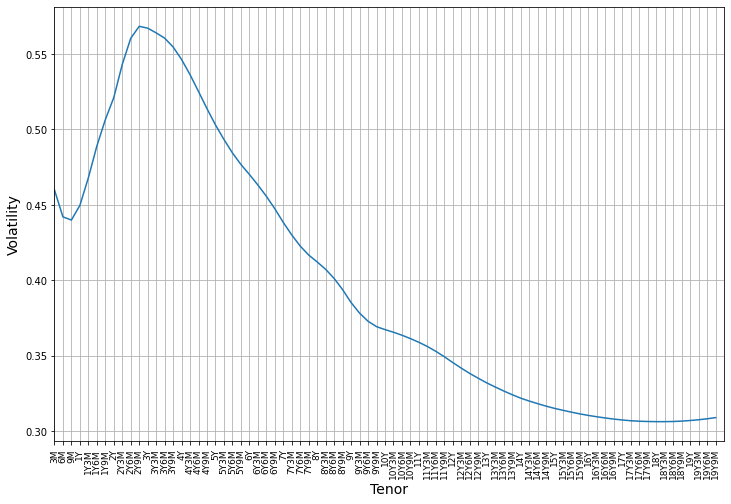
\includegraphics[width=0.5\linewidth]{images/cap_vola}
	\end{center}
\end{frame}

\begin{frame}{Remarks on LFM and Cap Pricing}
	\begin{itemize}
		\item A possible explanation of the humped shape is obtained by segmenting the caplet market across three maturities, (see Rebonato, 2002)
		\begin{enumerate}
			\item \textbf{Very short end of the curve}: central banks nowadays clearly communicate their strategy so that their actions are largely anticipated, leading to low volatilities in this region;
			\item \textbf{6M to 12-18M}: market participants continuously assess their expectations of future monetary policy, this is the region where subject beliefs have largest impact;
			\item \textbf{Longer maturities}: lastly, the third segment is much more affected by structural, long-term
			changes in expectations related to inflation and real rates/real returns. Thus, these long-term concerns are more or less independent of short-term monetary policies and the forward rate volatility is relatively low at the long end of the curve.
		\end{enumerate}
	\end{itemize}
\end{frame}

\begin{frame}{Back to Calibration}
The calibration procedure can be summarized as follows:
\begin{enumerate}
	\item<1-> determine the implied volatilities of Cap/Floor by inverting the Black formula using the market quotes. Those are the $v_{T_{j-cap}}$ flat volatilities;
	\item<2-> recover the correct spot volatilities with a numerical procedure (i.e. \emph{bootstrap}) from Eq.~\ref{eq:spot_flat_vola};
	\item<3-> finally we can go back to the instantaneous parameter of the model through
	\begin{equation}
		v_{T_{i-1}-caplet}^2 =\cfrac{1}{T_{i-1}} \int_0^{T_{i-1}}\sigma^2_{i,j}dt%=\cfrac{1}{T_{i-1}}\sum_{j=1}^{i-1}\tau_{j-1,j}\sigma^2_{i,j}
	\end{equation}
	Note that different parametrizations of the instantaneous volatility $\sigma_{i,j}^2$ lead to different evolutions of its term-structures.
\end{enumerate}
\end{frame}

\begin{frame}{Financial Bootstrapping}
	\begin{itemize}
		\item Bootstrapping is a widely used technique to derive financial quantities from others available in the market.
		\item The algorithm relies on a set of contracts (bonds, swaps, caps,\ldots) with different maturities from which, with an iterative procedure, the unknown variable can be extracted.
		\item As an example let's consider a set of coupon bearing bonds with annual frequency and with maturities ranging from 1 to 5Y. From the market we get their current quotes. We can write the following system of equations:
		\begin{equation*}
			\begin{cases}
			NPV(r_1) = P_1 \implies r_1 = NPV^{-1}(P_1)\quad\text{(iter 1)}\\
			NPV(r_1, r_2) = P_2 \implies r_2 = NPV^{-1}(r_1, P_2)\quad\text{(iter 2)} \\
			NPV(r_1, r_2, r_3) = P_3 \implies r_3 = NPV^{-1}(r_1, r_2, P_3)\quad\text{(iter 3)} \\
			NPV(r_1, r_2, r_3, r_4) = P_4 \ldots\\
			NPV(r_1, r_2, r_3, r_4, r_5) = P_5\ldots
			\end{cases}
		\end{equation*}
	\end{itemize}
\end{frame}

\begin{frame}{Caplet Volatility Bootstrapping \colablink{https://colab.research.google.com/drive/1v6RwkYOdFfE05kfax2h8A10AvBUUIZho}}
Let's \emph{strip} caplet volatilities from the following cap (\emph{flat}) volatilities (they referred to caps with 0.013 strike over EURIBOR-6M).
\begin{columns}
	\column{0.5\linewidth}
	\begin{center}
\begin{tabular}{|c|c|}
	\hline
	Maturity & Volatility \\
	\hline
	1y & $44\%$ \\
	\hline
	2y & 45\% \\
	\hline
	3y & 44\% \\
	\hline
	4y & 41\% \\
	\hline
	5y & 39\% \\
	\hline
\end{tabular}
\end{center}
	\column{0.5\linewidth}
\begin{center}
\begin{tabular}{|c|c|}
	\hline
	Pillar & Rate \\
	\hline
	3m & 0.0002 \\
	\hline
	6m & 0.0007 \\
	\hline
	12m & 0.0025 \\
	\hline
	2y & 0.0070 \\
	\hline
	3y & 0.0100 \\
	\hline
	5y & 0.0162 \\
	\hline
\end{tabular}
\end{center}
\end{columns}
\end{frame}

\begin{frame}{Caplet Volatility Bootstrapping}
\begin{enumerate}
\item We start with the nearest instruments, i.e. the spot starting caplet with $6m$ maturity. For maturities shorter than the first quoted value we consider the volatility constant hence:
\begin{equation*}
\sigma^{spot}_{6m}= \sigma^{spot}_{6m,1y} = \color{green}{\sigma^{flat}_{1y}}
\end{equation*}

\item Let’s now price the $1y$ forward starting caplet with $6m$ maturity. Since market cap volatilities are quoted assuming \textbf{no-arbitrage} opportunity we can build the forward starting caplet as the difference of two caps:

\begin{equation*}
\begin{gathered}
\textbf{Cpl}_{1y,1y6m}(\sigma^{spot}_{1y6m})=\textbf{Cap}_{1y6m}-\textbf{Cap}_{1y} \\[0.3cm]
\textbf{Cap}_{1y6m}=\textbf{Cpl}_{6m}(\textcolor{maincolor}{\sigma^{flat}_{1y6m}}) + \textbf{Cpl}_{6m,1y}(\textcolor{maincolor}{\sigma^{flat}_{1y6m}}) + \textbf{Cpl}_{1y,1y6m}(\textcolor{maincolor}{\sigma^{flat}_{1y6m}}) \\[0.3cm]
\textbf{Cap}_{1y}=\textbf{Cpl}_{6m}(\textcolor{green}{\sigma^{flat}_{1y}}) + \textbf{Cpl}_{6m,1y}(\textcolor{green}{\sigma^{flat}_{1y}})
\end{gathered}
\end{equation*}
\end{enumerate}
\end{frame}

\begin{frame}{Caplet Volatility Bootstrapping}
\begin{columns}
\column{0.5\linewidth}
Unfortunately the $18m$ volatility is NOT quoted on the market, so we can:
\begin{itemize}
	\item assume for the sake of simplicity that the volatility remains constant between $1y$ and $2y$ caps;
	\item use an interpolation method such as linear or cubic spline to get the $1y6m$ cap volatility.
\end{itemize}
\column{0.5\linewidth}
\begin{center}
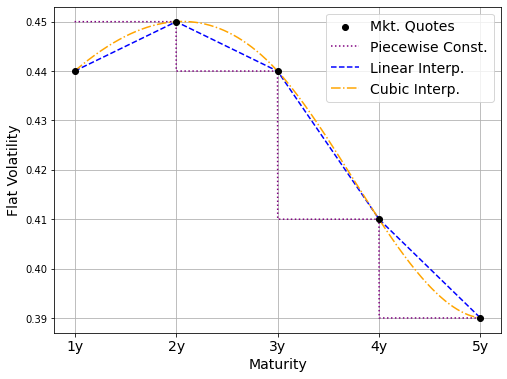
\includegraphics[width=0.8\linewidth]{images/flat_volatilities}
\end{center}
\end{columns}
Once "estimated" $\sigma^{flat}_{1y6m}$ We will be able to solve a single volatility from previous Equation by using a Newton-Raphson or Brent method.
\end{frame}

\begin{frame}{Caplet Volatility Bootstrapping}
\begin{enumerate}
\setcounter{enumi}{2}
\item We can apply the same method for the $1y6m$ forward starting caplet to get the volatility, $\sigma^{flat}_{2y}$ is quoted so no interpolation is needed here.

\begin{equation*}
\begin{gathered}
\textbf{Cpl}_{1y6m,2y}(\sigma^{spot}_{2y})=\textbf{Cap}_{2y}-\textbf{Cap}_{1y6m} \\[0.3cm]
\textbf{Cap}_{2y}=\textbf{Cpl}_{6m}(\textcolor{green}{\sigma^{flat}_{2y}}) + \textbf{Cpl}_{6m,1y}(\textcolor{green}{\sigma^{flat}_{2y}}) + \ldots + \textbf{Cpl}_{1y6m,2y}(\textcolor{green}{\sigma^{flat}_{2y}}) \\[0.3cm]
\textbf{Cap}_{1y6m}=\textbf{Cpl}_{6m}(\textcolor{green}{\sigma^{flat}_{1y6m}}) + \textbf{Cpl}_{6m,1y}(\textcolor{green}{\sigma^{flat}_{1y6m}}) + \textbf{Cpl}_{1y,1y6m}(\textcolor{green}{\sigma^{flat}_{1y6m}})
\end{gathered}
\end{equation*}

\item Keep iteratively to solve for all the remaining volatilities using the very same technique.
\end{enumerate}
\end{frame}

\begin{frame}[fragile]{Caplet Volatility Bootstrapping}
	\begin{center}
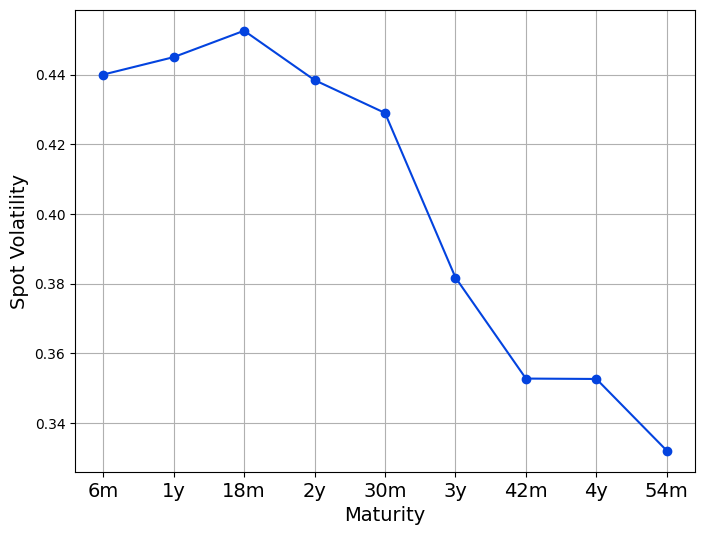
\includegraphics[width=0.65\linewidth]{images/spot_volatilities}
	\end{center}
\end{frame}

\begin{frame}{Instantaneous Volatility of Forward Rates}
	\begin{itemize}
		\item From \cref{eq:caplet_black_vol} ($v_i^2 = \frac{1}{T_{i-1}}\int_0^{T_{i-1}}\sigma_i^2(t)dt
		$) it is clear how it is impossible to uniquely determine the instantaneous volatility $\sigma_i(t)$ as there exist plenty of functions that would integrate to $v_i$.
		\item It is common to assume the $F_k$ has a \emph{piecewise-constant} volatility $\sigma_i(t)$ (constant in each maturity-expiry interval $i$).
		\item Nevertheless, to reduce the number of parameters of the model, further assumptions can be made (below some examples):
	\end{itemize}
	\begin{center}
		\begin{tabular}{|c|c|}
			\hline
			function of time-to-maturity & $\eta_{i-(\beta(t)-1)}$ \\ \hline
			constant regardless of $t$ & $s_i$ \\ \hline
			%most general parametrization & $\Phi_i\Psi_{\beta(t)}$ \\ \hline
			maturity/time to maturity & $\Phi_i\Psi_{i-(\beta(t)-1)}$ \\ \hline
			parametric & $[a(T_{i-1}-t) + d]e^{-b(T_{i-1}-t)} + c$ \\ \hline
			%parametric 2 & $\Phi_i\left([a(T_{i-1}-t) + d]e^{-b(T_{i-1}-t)} + c\right)$ \\ \hline
		\end{tabular}
	\end{center}
\end{frame}

\begin{frame}{Functional Form for Instantaneous Volatility}
	One commonly used function is the parametric form specified in the previous table. This ensure a smooth term structure:

	\[ \sigma_i(t) = [a(T_i - t) + b]e^{-c(T_i - t)} + d \]

	\begin{itemize}
		\item The parameters $\{a, b, c, d\}$ are calibrated to the entire Cap market simultaneously.
		\item This form captures the empirical reality that volatility often peaks for 2-3 year tenors before decaying (the hump).
		\item Finally it ensures that as time $t$ progresses in the Monte Carlo simulation, the volatility of the forward rates evolves realistically.
	\end{itemize}
\end{frame}

\section{Correlated Brownian Motions}
\begin{frame}{Instantaneous and Terminal Correlation}
	\begin{itemize}
		\item<1-> Let's consider now payoffs whose value depends on more than one rate simultaneously (e.g. swaptions).
		\item<1-> The price of these contracts depends on the \emph{terminal correlation} between different forward rates.
		\item<2-> In the derivation of the market models it has been assumed that each forward rate $F_i$ was driven by a different Brownian motion $W_i$ and that each Brownian motion is instantaneously correlated
		\begin{equation}
			< dW_i dW_j> = \rho_{ij} dt
		\end{equation}
		\item<3-> We need to understand how this correlation translates into the terminal correlation between rates.
	\end{itemize}
\end{frame}

\begin{frame}{Instantaneous and Terminal Correlation}
	%\begin{itemize}
	%\item For calibrating a LIBOR market model, instantaneous
	%  correlation is modeled. However, for pricing correlation-sensitive products, terminal correlation is used.
	%\item Define an $n$-dimensional LFM with $m$ factors:
	%\begin{equation*}
	%	\frac{df_i}{f_i} = \mu_i dt + \sigma_i \sum_{k=1}^m b_{ik}dZ_k
	%\end{equation*}
	%with $b_k=\frac{\sigma_{ik}}{\sqrt{\sum_{k=1}^m\sigma_{ik}^2}}$

	\begin{block}{Definition}
			The \textcolor{maincolor}{instantaneous correlation} is a quantity summarizing the degree of “dependence” between \textcolor{maincolor}{changes} of different forward rates.
			\begin{equation*}
					\rho_{ij} = \frac{dF_i(t) dF_j(t)}{\text{Std}(dF_i(t))\text{Std}(dF_j(t))}
				\end{equation*}
			%where $Std$ denotes the standard deviation conditional on the information available at time $t$ at which the change occurs.
			%The instantaneous correlation of the LIBOR rates $L(t, T_{i-1}, T_i)$ and $L(t, T_{j-1}, T_j)$ is given by the correlation of the increments of the Brownian motions:
			%\begin{equation*}
			%\rho_{i,j}(t) = \sum_{k=1}^m b_{i,k}b_{j,k}, \quad i,j=1,\ldots,n
			%\end{equation*}
			%From this formula it is clear that indeed the instantaneous correlation ρ is related to changes dF in for- ward rates. Instead,
			The \textcolor{maincolor}{terminal correlation} is a quantity summarizing the degree of “dependence” between two different forward rates at a given  \textcolor{maincolor}{terminal time-instant}. Typically, the $T_1$ terminal correlation between $F_i$ and $F_j$ is the correlation between $F_i(T_1)$ and $F_j(T_1)$.
		\end{block}
	\uncover<2->{Is this terminal correlation completely determined by the instantaneous correlations $\rho_{ij}$ between $W_i$ and $W_j$ ?}
	%\begin{block}{Definition}
	%The terminal correlation of the LIBOR rates$L(t, T_{i-1}, T_i)$ and $L(t, T_{j-1}, T_j)$ is given by
	%\begin{equation*}
	%\tilde{\rho}_{i,j}(t) = %\frac{\int_o^t\sigma_i(u)\sigma_j(u)\rho_{i,j}(u)du}{\sqrt{\int_0^t\sigma_i(u)^2du\int_o^t\sigma_j(u)^2du}}
	%\end{equation*}
	%\end{block}
	%\end{itemize}
\end{frame}

\begin{frame}{Swaption Calibration}
	The "Model" volatility of the Swaption that we compare against the Market is:

	\[ \sigma_{Swap}^2 \approx \sum_{i=m}^{n-1} \sum_{j=m}^{n-1} w_i w_j \sigma_i \sigma_j \rho_{ij} \]

	$\sigma_i,j$ have been determined from the caps.
	A Swap Rate $S_{m,n}$ is a weighted average of forward rates $F_i$. To calibrate, we calculate the sensitivity weights $w_i$:

\[ w_i = \frac{\tau_i P(0, T_{i+1})}{\sum_{k=m}^{n-1} \tau_k P(0, T_{k+1})} \]

	The \emph{Rebonato Weights} represent the "contribution" of each Libor rate to the total value of the swap's floating leg.
\end{frame}

\begin{frame}{Calibrating Correlation ($\rho$)}
	From the market swap rate variance (previous formula) we can now calibrate the correlation between forward rates.
	To reduce the number of parameters, we often assume:
	\[ \rho_{ij} = \exp(-\beta |T_i - T_j|) \]
	\begin{itemize}
		\item If $\beta$ is high, rates are decoupled (low correlation).
		\item If $\beta = 0$, all rates move perfectly together.
		\item These are found by minimizing the error across a \textit{matrix} of Swaptions with different maturities and tenors.
	\end{itemize}
\end{frame}

\begin{frame}{Two-Factor Correlation Model}
	The standard exponential decay $e^{-\beta \Delta T}$ often fails to capture long-term curve dynamics. We introduce a \textbf{Correlation Floor} $L$:

	\[ \rho_{ij} = L + (1 - L)e^{-\beta |T_i - T_j|} \]

	\begin{itemize}
		\item \textbf{Parameter $L$ (Level):} represents the "Parallel Shift." Even for rates very far apart, correlation never drops below $L$.
		\item \textbf{Parameter $\beta$ (Decay):} represents the "Twist." How quickly the curve decouples as tenors diverge.
	\end{itemize}
	\vspace{0.3cm}
\end{frame}
















%\begin{frame}{Calibrating Volatility ($\sigma$)}
%	Under the LFM, the Caplet volatility $\sigma_{Mkt, i}$ and the LFM instantaneous volatility $\sigma_i(t)$ are related via:
%	\[ \sigma_{Mkt, i}^2 T_i = \int_0^{T_i} \sigma_i(t)^2 dt \]
%
%	\textbf{Approaches:}
%	\begin{itemize}
%		\item \textbf{Piecewise Constant:} $\sigma_i(t)$ is constant between tenor dates. This allows an exact match to the Caplet term structure.
%		\item \textbf{Parametric Form:} e.g., $\sigma_i(t) = [a(T_i - t) + b]e^{-c(T_i - t)} + d$. This "smooths" the volatility across tenors to avoid numerical instability.
%	\end{itemize}
%\end{frame}


\subsection{Confidence Interval}
\begin{frame}{Confidence Interval}
	\begin{itemize}
			\item<1-> Consider a general payoff at time $T$, $\Pi(T)$, depending on a vector of spanning forward LIBOR rates $\bm{\tilde{F}}(t)$. %, for $t \in [0, T]$, where typically $T$ is smaller than or equal to the expiry of the first forward rate.
			\item<2-> We simulate various scenarios of $\Pi(T)$ under the $T$-forward measure. Let $m$ be the number of simulated paths, the Monte Carlo price of the payoff is
			\begin{equation*}
					\expect{Q}[D(0,T)\Pi(T)] = P(0,T)\mathbb{E}^T[\Pi(T)]\approx \frac{P(0,T)}{m}\sum_{j=1}^{m}\Pi_j(T)
				\end{equation*}
			\item<3-> Since $\Pi_1(T), \Pi_2(T),\ldots$ is a sequence of realizations of i.i.d. random variables distributed as $\Pi(T)$, the \textcolor{maincolor}{Central Limit Theorem} tell us that for $m\rightarrow\infty$
			\begin{equation*}
					\cfrac{\sum_{j=1}^{m}\Pi_j(T)-\mathbb{E}^T[\Pi(T)]}{\sqrt{m} \text{Std}(\Pi(T))}\rightarrow \mathcal{N}(0,1)
				\end{equation*}
		\end{itemize}
\end{frame}

\begin{frame}{Confidence Interval}
	\begin{columns}
			\column{0.6\linewidth}
			\begin{itemize}
					\item<1-> Thus, for large $m$, the following approximation holds
					\begin{equation*}
							\frac{\sum_{j=1}^{m}\Pi^j}{m}-\mathbb{E}^T[\Pi]\approx \frac{\text{Std}(\Pi)}{\sqrt{m}}\mathcal{N}(0,1)
						\end{equation*}
				\end{itemize}
			\column{0.4\linewidth}
			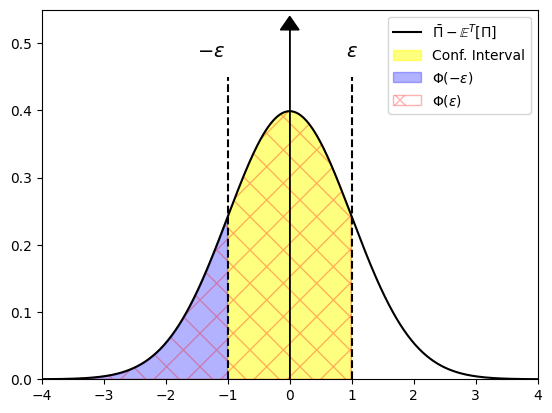
\includegraphics[width=0.9\linewidth]{images/epsilon}
		\end{columns}
	\begin{itemize}
			\item<2-> The probability that the MC estimate is closer than $\epsilon$ to the true price is
			\begin{equation*}
					P\left(\bigg|\frac{\sum_{j=1}^m\Pi_j}{m}-\mathbb{E}^T[\Pi]\bigg|<\epsilon\right) = P\left(|\mathcal{N}(0,1)|<\epsilon\frac{\sqrt{m}}{\text{Std}(\Pi)}\right) =
					2\Phi\left(\epsilon\frac{\sqrt{m}}{\text{Std}(\Pi)}\right)-1
				\end{equation*}
			where $\Phi$ denotes the c.d.f. of the standard Gaussian distribution.
			\begin{equation*}
					P(|x|<\epsilon) = \Phi(\epsilon) - \Phi(-\epsilon) = \Phi(\epsilon) - (1 - \Phi(\epsilon)) = 2\Phi(\epsilon) - 1
				\end{equation*}
		\end{itemize}
\end{frame}

\subsection{Variance Reduction}
\begin{frame}{Monte Carlo Variance Reduction}
	To reduce the confidence interval without running too many simulations, i.e. reduce the sample variance, without increasing $m$, the \textcolor{maincolor}{control variate technique} can be used.
	\pause
	\begin{enumerate}
			\item<2-> Consider another payoff $\Pi_{an}$ which we can be evaluated analytically, whose expectation is denoted by $\mathbb{E}[\Pi_{an}] = \pi_{an}$, and simulate it together with $\Pi$ under the same scenarios.% for $\bar{F}$.
			\item<3-> Define an unbiased estimator for $\mathbb{E}[\Pi]$ as the sample mean of the random variable
			\begin{equation*}
					\Pi_c(\gamma) = \Pi + \gamma(\Pi_{an} - \pi_{an})
				\end{equation*}
			Hence $\Pi_c(\gamma)$ has expectation $\mathbb{E}[\Pi]$ and variance
			\begin{equation*}
					\text{Var}(\Pi_c(\gamma)) = \text{Var}(\Pi) + \gamma^2 \text{Var}(\Pi_{an}) + 2\gamma \text{Cov}(\Pi, \Pi_{an})
				\end{equation*}
		\end{enumerate}
\end{frame}

\begin{frame}{Monte Carlo Variance Reduction}
	\begin{enumerate}\addtocounter{enumi}{2}
			\item This can be minimized by choosing the appropriate $\gamma$ $\left(\text{from }\frac{\partial \text{Var}(\Pi_c)}{\partial\gamma}=0\right)$
			\begin{equation*}
					\gamma^* = -\frac{\text{Cov}(\Pi, \Pi_{an})}{\text{Var}(\Pi_{an})} = -\frac{\text{Corr}(\Pi, \Pi_{an})\text{Std}(\Pi)}{\text{Std}(\Pi_{an})}, \quad \left(\text{Corr}_{XY}=\frac{\text{Cov}_{XY}}{\text{Std}_X \text{Std}_Y}\right)
				\end{equation*}
			and the minimum variance of $\Pi_c$ is computed as
			\begin{equation*}
					\text{Var}(\Pi_c(\gamma^*)) = \text{Var}(\Pi)(1 - \text{Corr}(\Pi, \Pi_{an})^2)
				\end{equation*}
			that is \textcolor{maincolor}{smaller than the variance of $\Pi$}. Moreover, the \textcolor{maincolor}{larger the correlation between $\Pi$ and $\Pi_{an}$ the larger the difference between the two variances}.
		\end{enumerate}
\end{frame}

\begin{frame}{Monte Carlo Variance Reduction}
	\begin{enumerate}\addtocounter{enumi}{3}
			\item<1-> Moving to the standard deviation
			\begin{equation*}
					\text{Std}(\Pi_c(\gamma^*)) = \text{Std}(\Pi) \sqrt{1 - \text{Corr}(\Pi, \Pi_{an})^2}
				\end{equation*}
			the variance reduction will increase with the correlation between $\Pi$ and $\Pi_{an}$.
			\item<2-> Now if we consider the confidence interval for $\Pi_c$
			\begin{equation*}
					98\% C.L. =\left[\Pi_c(\gamma,m) - 2.33\cdot\frac{\text{Std}(\Pi_c)}{\sqrt{m}};\Pi_c(\gamma,m) + 2.33\cdot\frac{\text{Std}(\Pi_c)}{\sqrt{m}}\right]
				\end{equation*}
			we get a narrower width by a factor of
			\begin{equation*}
					\sqrt{1 - \text{Corr}(\Pi, \Pi_{an}; m)^2}
				\end{equation*}
		\end{enumerate}
		This technique is quite general and the \textcolor{maincolor}{choice of $\Pi_{an}$ is theoretically free}.
		In the case of the pricing of swaptions in the LFM, we select as $\Pi_{an}$ one of the simplest choice, the Black price of the swaption.
\end{frame}

%\begin{frame}{Monte Carlo Variance Reduction}
%	\begin{itemize}
%			\item<1-> This technique is quite general and the \textcolor{maincolor}{choice of $\Pi_{an}$ is theoretically free}.
%			\item<2-> In the case of the pricing of swaptions in the LFM, we select as $\Pi_{an}$ one of the simplest choice, the Black price of the swaption.
%			\item<3-> Consider the payoff of such portfolio where the $K_i = F_i(0)$ and rewrite it by a change of measure as follows:
%			\begin{equation*}
%					\begin{aligned}
%							\textbf{FRAs} = &\expect{Q}\left[D(0,T_\alpha)\sum_{i=\alpha+1}^\beta P(T_\alpha,T_i)\tau_i(F_i(T_\alpha) - F_i(0))\right] = \\
%							&=\mathbb{E}^j\left[\frac{P(0,T_j)}{P(T_\alpha,T_j)}\sum_{i=\alpha+1}^\beta P(T_\alpha,T_i)\tau_i(F_i(T_\alpha) - F_i(0))\right] = \\
%							& = P(0,T_j)\mathbb{E}^j\left[\frac{\sum_{i=\alpha+1}^\beta P(T_\alpha,T_i)\tau_i(F_i(T_\alpha) - F_i(0))}{P(T_\alpha,T_j)}\right]
%						\end{aligned}
%				\end{equation*}
%		\end{itemize}
%\end{frame}
%
%\begin{frame}{Monte Carlo Variance Reduction}
%	\begin{itemize}
%			\item<1-> Thus we can set
%			\begin{equation*}
%					\Pi_{an}(T_\alpha) = \frac{\sum_{i=\alpha+1}^\beta P(T_\alpha,T_i)\tau_i(F_i(T_\alpha) - F_i(0))}{P(T_\alpha,T_j)}
%				\end{equation*}
%			whose price at time $T_\alpha = 0$ is $\pi_{an} = 0$.
%			\item<2-> Indeed, the payoff $\Pi_{an}(\cdot)$ is a sum of traded assets divided by $P(\cdot, T_j)$, hence it is a martingale under the $T^j$-forward measure $\mathbb{Q}^j$, which implies that
%
%			\begin{equation*}
%					\mathbb{E}^j[\Pi_{an}(T_\alpha)] = \mathbb{E}^j[\Pi_{an}(0)] = 0
%				\end{equation*}
%		\end{itemize}
%\end{frame}
%
%\begin{frame}{5. Variance Reduction: Control Variates}
%	To reduce the width of the Confidence Interval $\frac{\text{Std}(\Pi)}{\sqrt{m}}$, we introduce a control variate $\Pi_{an}$ with a known expectation $\pi_{an}=0$.
%
%	\[ \Pi_c(\gamma) = \Pi + \gamma(\Pi_{an} - 0) \]
%
%	\textbf{Implementation in LFM:}
%	\begin{itemize}
	%		\item Use a portfolio of FRAs as $\Pi_{an}$ since they are martingales under their respective measures.
	%		\item \textbf{Optimal $\gamma^*$:} Calculated to minimize variance: $\gamma^* = -\frac{\text{Cov}(\Pi, \Pi_{an})}{\text{Var}(\Pi_{an})}$.
	%		\item \textbf{Efficiency:} The variance is reduced by a factor of $(1 - \text{Corr}(\Pi, \Pi_{an})^2)$. High correlation between the Swaption and the FRA portfolio is key.
	%	\end{itemize}
%\end{frame}
%
%\begin{frame}{The Role of Correlation and $\beta^*$}
%	We found that the correlation between a Swaption and a single Caplet is often imperfect ($\rho \approx 0.66$).
%
%	\begin{block}{Optimizing the Correction}
%		Using a fixed $\beta=1$ assumes a 1:1 relationship. If correlation is low, this increases variance. We must use:
%		\[ \beta^* = \frac{Cov(Y, X)}{Var(X)} = \rho_{YX} \frac{\sigma_Y}{\sigma_X} \]
%	\end{block}
%
%	\textbf{Observation:} A $\beta^* < 1$ "dampens" the control variate correction to account for the fact that the terminal rate doesn't perfectly represent the entire swap basket.
%\end{frame}





%
%
%
%
%
%
%
%
%%\begin{frame}{Advanced Variance Reduction: Control Variates}
%%	Monte Carlo error is $O(1/\sqrt{M})$. To achieve high precision, we use:
%%	\[ Y_{CV} = Y_{LFM} + \beta^*(E[X] - X) \]
%%
%%	\textbf{Why it works in LFM:}
%%	\begin{itemize}
%%		\item We use the \textbf{Terminal Caplet} as our control $X$.
%%		\item Since $L_{N-1}$ has no drift, its analytical Black-76 price ($E[X]$) is exact.
%%		\item If the simulation over-samples high interest rate paths, both $Y_{LFM}$ and $X$ will be high. The subtraction $(E[X] - X)$ cancels out this sampling noise.
%%	\end{itemize}
%%\end{frame}



%\section{LFM Implementation Pipeline}
%
%\begin{frame}{1. From Caplet Volatilities to Instantaneous $\sigma_i(t)$}
%	To simulate the forward rates $F_i(t)$, we must decompose the market-bootstrapped Caplet volatilities $v_i$ into instantaneous volatility functions $\sigma_i(t)$.
%
%	\begin{itemize}
%		\item \textbf{The Constraint:} The model must recover market prices: $v_i^2 T_{i-1} = \int_0^{T_{i-1}}\sigma_i^2(t)dt$.
%		\item \textbf{Parametric Form:} To ensure a smooth term structure and reduce parameters, we often assume:
%		\[ \sigma_i(t) = [a(T_{i-1} - t) + d]e^{-b(T_{i-1} - t)} + c \]
%	\end{itemize}
%
%	\begin{center}
%		\footnotesize
%		\begin{tabular}{|l|c|l|}
%			\hline
%			\textbf{Approach} & \textbf{Form} & \textbf{Property} \\ \hline
%			Piecewise Constant & $\sigma_{i, \beta(t)}$ & Exact match to all Caplets \\ \hline
%			Time-to-maturity & $\eta_{i-(\beta(t)-1)}$ & Stationary volatility structure \\ \hline
%			Full Parametric & $f(T, t; a,b,c,d)$ & Captures the empirical "hump" \\ \hline
%		\end{tabular}
%	\end{center}
%\end{frame}
%
%\begin{frame}{2. Instantaneous vs. Terminal Correlation}
%	\begin{itemize}
%		\item \textbf{Instantaneous correlation} $\rho_{ij}$ drives the dependence between increments $dW_i$ and $dW_j$.
%		\item \textbf{Terminal correlation} (at $T_1$) depends on \textit{both} $\rho_{ij}$ and how $\sigma_i(t)$ is distributed over time.
%	\end{itemize}
%
%	\begin{exampleblock}{Sensitivity Example}
%		Consider two ways to decompose the same Caplet $v_i$ into $\sigma_{i,1}$ and $\sigma_{i,2}$:
%		\begin{center}
%			\begin{tabular}{|c|c|c|c|c|}
%				\hline
%				& $\sigma_{2,1}$ & $\sigma_{3,1}$ & $\sigma_{2,2}$ & $\sigma_{3,2}$ \\ \hline
%				Case A & 0.5 & 0.1 & 0.1 & 0.5 \\ \hline
%				Case B & 0.1 & 0.1 & 0.5 & 0.5 \\ \hline
%			\end{tabular}
%		\end{center}
%		Even with identical $\rho_{ij}$, Case A yields an expectation $\approx 1.8 \cdot 10^{-3}$ while Case B yields $\approx 2.3 \cdot 10^{-4}$. \textbf{The path of instantaneous volatility matters for Swaptions.}
%	\end{exampleblock}
%\end{frame}
%
%
%
%\begin{frame}{Terminal Correlation}
%\begin{itemize}
%\item<1-> In general the terminal correlation between different forward rates depends not only on the introduced instantaneous correlations, \emph{but also on the way the “total” (caplet volatility) is “distributed” in instantaneous volatility (on $\sigma_{k,\beta(t)}$)}.
%\item<1-> Keeping the same instantaneous correlations and decomposing $v_i$ in two different ways leads to different correlations between $F_i$.
%%This elementary and fundamental feature of terminal correlation was noticed and pointed out in Rebonato (1998, 1999d).
%\item<2-> Also, while the instantaneous correlation does not depend on the particular probability measure, \emph{the terminal correlation does.}
%\item<3-> The Girsanov theorem establishes that the instantaneous covariance structure is the same for all the equivalent measures under which a process can be expressed, so that the particular measure under which we work makes no difference.
%\item<4-> This is not the case for terminal correlation.
%\end{itemize}
%\end{frame}
%
%\begin{frame}{Terminal Correlation: an Example}
%\begin{itemize}
%\item<1-> Consider a payoff $\Pi = (\log(F_3(T_1))-\log(F_3(T_0)))(F_2(T_1)-F_2(T_0))$ where $T_0>0$, $T_1=2T_0$, taking the measure $\mathbb{Q}^2$ under which $F_2$ is a martingale
%\begin{equation*}
%\begin{gathered}
%dF_2(t) = \sigma_{2,\beta(t)}F_2(t)dW_2(t)\\
%dF_3(t) = \cfrac{\tau_3\sigma^2_{3,\beta(t)}F_3^2(t)}{1+\tau_3F_3(t)}dt + \sigma_{3,\beta(t)}F_3(t)dW_3(t)
%\end{gathered}
%\end{equation*}
%\item<2-> As an example consider the payoff expectation, which results to be a terminal correlation dependent quantity
%\begin{equation}
%\begin{aligned}
%\mathbb{E}^2[\Pi] & = F_2(0)\rho_{2,3}\int_0^{T_1}\sigma_{2,\beta(t)}\sigma_{3,\beta(t)}dt = \\
%
%&  = F_2(0)\rho_{2,3}(\sigma_{2,1}\sigma_{3,1}T_0+\sigma_{2,2}\sigma_{3,2}\tau_{0,1})
%\end{aligned}
%\label{eq:terminal_correlation_ex}
%\end{equation}
%\end{itemize}
%\end{frame}
%
%\begin{frame}{Terminal Correlation: an Example}
%\begin{itemize}
%\item<1-> Now from what we have said any \emph{caplet} price involving the rates $F_2$ and $F_3$ would depend only on the average volatilities $v_2^2$ and $v_3^2$: \textcolor{maincolor}{no matter how $\sigma_{k,t}$ are chosen} the Black formula gives the same result.
%\item<2-> Contrary from \cref{eq:terminal_correlation_ex} it is clear that there is a dependency on the instantaneous volatilities.
%\item<3-> Consider the cases where $\tau=T_i - T_{i-1}=0.5$, $F_2(0)=F_3(0)=0.05$, $\rho_{2,3}=0.75$, $\sigma_{3,3}=0.1$ and
%\begin{center}
%\begin{tabular}{|c|c|c|c|}
%\hline
%$\sigma_{2,1}$ & $\sigma_{3,1}$ & $\sigma_{2,2}$ & $\sigma_{3,2}$ \\ \hline
%0.5 & 0.1 & 0.1 & 0.5 \\ \hline
%0.1 & 0.1 & 0.5 & 0.5 \\ \hline
%\end{tabular}
%\end{center}
%\item<3-> In the first case the result is $1.875\cdot10^{-3}$ while in the latter $2.343\cdot10^{-4}$.
%\end{itemize}


\begin{frame}{Decorrelation}
	In the context of the Libor Forward Model (LFM) and the Two-Factor Correlation model we discussed, decorrelation refers to the phenomenon where forward rates of different tenors do not move perfectly in sync.

	In a financial model, if $\rho_{ij}=1$, the rates are perfectly correlated (they only move up or down together in a parallel shift). Decorrelation is the "slack" or "twist" in the curve.

	Recall the correlation structure: $\rho_{ij}=L+(1-L)e^{-\beta|T_i-T_j|}$, $\beta$ is the "decorrelation speed."

	If $\beta>0$, then as the distance between two tenors ($|T_i-T_j|$) increases, the correlation $\rho_{ij}$ drops.

	$L$ prevents "total decorrelation," ensuring that even the 1Y and 30Y rates maintain some fundamental connection.
\end{frame}

\begin{frame}{Impact on Swaption Pricing}
	A Swaption is an option on a weighted basket of forward rates. Decorrelation is a primary driver of the basket's total volatility.

	If all rates are perfectly correlated, the volatility of the swap rate is simply the weighted average of the individual volatilities.

	If rates decorrelate, they can move in opposite directions. This "hedges" the basket, resulting in a lower swap rate volatility even if individual caplet volatilities remain high.

	By comparing the bootstrapped caplet volatilities to market swaption prices, you can "spot" whether the market is pricing in a high degree of decorrelation (a "twisting" curve) or low decorrelation (a "parallel" shifting curve).
\end{frame}

\begin{frame}{Relation to the Terminal Measure Drift}

	Looking at the \textbf{drift} term in the Forward Rate SDE it is apparent how the decorrelation ($\rho{ij}$) directly scales it.

	If rates are highly decorrelated (low $\rho{ij}$), the "no-arbitrage" pull (the drift) exerted by the numeraire is weaker. If you assume perfect correlation when the market is actually decorrelated, your Monte Carlo simulation will overstate the drift, leading to biased prices.

	Decorrelation can be managed via PCA: 1st Factor (Level): 90\% of movement (Perfect correlation), 2nd Factor (Slope/Twist): this is where decorrelation happens. One end of the curve goes up while the other goes down, 3rd Factor (Curvature/Butterfly): further decorrelation of the belly of the curve relative to the wings.
\end{frame}


%% \subsection{Decorrelation}
%% %\begin{frame}{Correlated Brownian Motions}
%% %  \begin{itemize}
%% %  \item<1-> Correlation is a linear measure of dependency between random variables. Given two random variables $X$ and $Y$, it is given by
%% %  	\begin{equation*}
%% %  		\rho_{X,Y} = \frac{\mathbb{E}((X-\mathbb{E}(X))(Y-\mathbb{E}(Y))}{\sigma_X \sigma_Y}
%% %  	\end{equation*}
%% %  \item<2-> In the LFM, we can assume that the Brownian motions driving the dynamics of forward rate are correlated
%% %    \begin{equation*}
%% %      <dZ_t^{T^i}, dZ_t^{T^i}> = \rho dt
%% %    \end{equation*}
%% %  \item<3-> This model feature is included because the value of a swaption at maturity is influenced by the joint distribution of forward rates and thus by the correlation amongst them.
%% %  \item<4-> For example, since the underlying in a swaption is a swap rate which in turn is a weighted average of forward rates, we expect the price of a swaption to increase if the forward rates become more correlated.
%% %  \end{itemize}
%% %\end{frame}
%
%% \begin{frame}{Correlated Brownian Motions}
%% 	\begin{itemize}
%% 	\item<1-> In short rate models, by modeling an "instant rate", there is only one source of randomness and all forward rates are perfectly correlated, $\rho_{ij}=1$.
%% 	\item<1-> This is a tight constraint on the dynamics of the forward rates.
%% 	\item<2-> When trying to improve these models, one of the objectives is to lower the correlation of the forward rates. Some authors refer to this objective as to \textcolor{maincolor}{decorrelation}.
%% 	\item<3-> In the LFM, this can be easily done by fine-tuning the corresponding parameters into the dynamics
%% 	\begin{equation*}
%% dF_k(t) = \sigma_kF_k\sum_{j=\alpha+1}^k\frac{\boxed{\rho_{kj}}\tau_j\sigma_jF_j}{1+\tau_jF_j}dt+\sigma_kF_k dW^\alpha_k
%% 	\end{equation*}
%% \end{itemize}
%% \end{frame}
%
%% \begin{frame}{Instantaneous Correlation}
%%   \begin{itemize}
%%   \item<1-> Instantaneous correlation can be estimated from historical market data.
%%   \begin{enumerate}
%% 	  \item first derive yield curves for some period of time in the past;
%% 	  \item then, forward curves may be calculated off the yield curves;
%% 	  \item finally the dependence between forward rate increments may be estimated.
%%   \end{enumerate}
%%   \item<2-> Many parametrizations functions have been introduced to express a given correlation matrix of forward rates in a functional form.
%%   \item<3-> This has several advantages: it is computationally convenient to work with an analytical formula. Noise (e.g. non-synchronous data or illiquidity) is removed by focusing on general properties of correlation. Furthermore, the correlation matrix rank can be controlled through the functional form.
%%   \item<4-> Anyway it would be nice to imply these correlations out of liquidly traded swaption prices.
%%   \end{itemize}
%% \end{frame}
%
%% %\begin{frame}{Correlation Parametrization}
%% %  \begin{itemize}
%% %  \item One property that is always implicitly present is time-homogeneity: correlation of forward rates does not depend on calendar time $t$, but only on the rates’ time to maturity $T_i-t$.
%% %  %\item An important aspect of these parameterizations is the number of parameters used to fit the market data. Most parameterizations advocate the use of few parameters that emphasize general properties of market correlation and prevent overfitting.
%% %  \item General requirements on an $M \times M$ correlation matrix $\rho$ are:
%% %	\begin{enumerate}
%% %		\item $\rho$ must be real and symmetric;
%% %		\item $\rho_{i,i}=1$ for $i = 1,\ldots, M$;
%% %		\item $\rho$ must be positive semi-definite such that can be decomposed into $\rho = BB^T$.
%% %	\end{enumerate}
%% %	\item Usually parameterizations are determined by minimizing the mean square error between historical market correlation and parameterized functional form.
%% %	\end{itemize}
%% %\end{frame}
%
%% \begin{frame}{Decorrelation}
%% \begin{itemize}
%% 	\item<1-> Generally, inferring instantaneous correlations from actively traded swaptions is desirable as they reflect current market conditions, thus not suffering from the backward-looking nature of historically estimated correlations.
%% 	\item<2-> There are however, also problems with implying correlations from the market. One such general problem, is that swaption prices depend on forward rate correlation \textbf{AND} volatility.
%% 	\item<3-> There is no liquidly traded fixed income derivative that solely depends on correlation, as opposed to caplets, which solely depend on volatility.
%% 	\item<4-> Another problem concerns the relationship between instantaneous and terminal correlations.
%% \end{itemize}
%% \end{frame}
%
%% \begin{frame}{Decorrelation}
%% 	\begin{itemize}
%% 	\item<1-> For terminal correlations, (Rebonato, 1998) shows that an appropriate quantity summarizing the amount of decorrelation between two stochastic variables from time 0 to time $t$ is
%% 	\begin{equation}
%% 		\tilde{\rho}_{ij}(t)=\frac{\int_0^t\sigma_i(u)\sigma_j(u)\rho_{ij}(u)du}{\sqrt{\int_0^t\sigma_i(u)^2 du\int_0^t\sigma_j(u)^2 du}}
%% 		\label{eq:terminal_correlation}
%% 	\end{equation}
%% 	\item<2-> From this equation, we see that the terminal correlation not only depends on the instantaneous correlation $\rho_{ij}$ but also on the instantaneous volatilities. Hence, even for perfectly instantaneously correlated random variables, $\rho_{ij}= 1$, terminal \textcolor{maincolor}{decorrelation} could be achieved by time-dependent instantaneous volatilities.
%% \end{itemize}
%% \end{frame}
%% %  \begin{itemize}
%% %  \item Is terminal correlation completely determined by the instantaneous correlations $\rho_{ij}$ between $W_i$ and $W_j$ ?
%% %  \item The answer is no, since terminal correlation also depends on the forward rate volatilities (caplet volatilities).
%% %  \item In particular it is important the choice of the function $\sigma(t)$ used to recover "average volatilities" through integration in $[0,T_i]$.
%% %  \item If \textcolor{maincolor}{instantaneous volatilities} are not constant, they have a significant impact on terminal correlation and can produce terminal \emph{decorrelation}, even in the case of perfect instantaneous correlation.
%% %  %\item Prices of correlation-sensitive products depend on terminal correlation, and thus instantaneous correlation and instantaneous volatility.
%% %  %\item It is important to note that there is no instrument that is sensitive solely to instantaneous correlation. Therefore, estimating correlation from a product that is sensitive to multiple factors is not straight-forward and can lead to ambiguous results.
%% %  \end{itemize}
%% %\end{frame}
%
%% \begin{frame}{An Example}
%% \begin{itemize}
%% 	\item<1-> Considering Rebonato's analytical formula for terminal correlation \cref{eq:terminal_correlation} it can be shown that in the case of piecewise-constant volatilities, terminal correlation is just the average correlation over the period.
%%   	\item<2-> Since the instantaneous volatilities are constant, they can be factored out from the integrals
%% 	  \begin{equation*}	    \tilde{\rho}_{ij}(t)=\frac{\cancel{\sigma_i}\cancel{\sigma_j}\int_0^t\rho_{ij}(u)du}{\sqrt{\cancel{\sigma_i^2}\cancel{\sigma_j^2} t^2}}= \frac{\int_0^t\rho_{ij}(u)du}{t}
%%   	\end{equation*}
%%   	which indeed leads to lower terminal correlation.
%%   	\item<3-> Swaption payoffs depend on the terminal correlation between several different forward rates which leads (Brigo and Mercurio, 2006) to the conclusion that swaption volatilities are more directly linked with terminal correlations rather than with instantaneous ones.
%%   \end{itemize}
%% \end{frame}
%
%% \begin{frame}{LFM Calibration to Swaptions}
%% \begin{itemize}
%% \item<1-> In case we are adopting the LFM, we need to find the instantaneous-volatility and correlation parameters in the LFM dynamics that reflect the swaptions prices observed in the market.
%
%% %Remark 6.17.1. (Possible misalignments in the swaption matrix).
%% %Usually, one should not completely rely on the swaption matrix provided
%% %by a single broker, and, in any case, one should not take it for granted. The
%% %problem is that the matrix is not necessarily uniformly updated. The most
%% %liquid swaptions are updated regularly, whereas some entries of the matrix
%% %refer to older market situations. This “temporal misalignment” in the swaptions matrix can cause troubles, since, when we try a calibration, the model parameters might reflect this misalignment by assuming “weird” values (we will see in Chapter 7 examples leading to imaginary and complex forwardrate volatilities).
%% \item<2-> The problem is incorporating as much information as possible from such a table into the LFM parameters.
%% \item<3-> The goal is to find the set of parameters $\bar{x}$ and $\bar{\theta}$ from volatility and correlation parametrizations such that to minimize the difference between the market prices and those computed from LFM.
%% \item<4-> However, if the number of swaptions is large, it is necessary to consider richer parametric forms, since the problem is over-dimensioned, although in this case care must be taken for the resulting market structures to be regular enough.
%% \end{itemize}
%% \end{frame}
%
%% %\begin{frame}{LSM Calibration to Swaptions}
%% %\begin{itemize}
%% %\item In the calibration process we should ask ourselves if we infer $\rho$ (correlation structure) itself from swaption market quotes or should we estimate it exogenously and impose it, leaving the calibration only to volatility parameters ?
%% %%\item Indeed, we might consider a time series of past interest-rate curves data, which are observed under the real world probability measure.
%% %%This would allow us, through interpolation, to obtain a corresponding time series for the particular forward LIBOR rates being modelled in our LIBOR model.
%% %%These series would be observed under the objective or real-world measure. Thanks to the Girsanov theorem this is not a problem, since instantaneous correlations, considered as instantaneous covariations between driving Brownian motions in forward rate dynamics, do not depend on the probability measure under which we are specifying the joint forward rate dynamics. Only the drifts depend on the measure. Then, by using some historical estimation technique, we can obtain an historical estimate of the instantaneous correlation matrix. This historical matrix ρ, or a stylized version of it, can
%% %%be considered as a given ρ for our LIBOR model, and the remaining free
%% %%parameters σ are to be used to calibrate market derivatives data at a given
%% %%instant. In this case (caps and) swaptions calibration will consist in finding
%% %%the σ’s such that the model (caps and) swaptions prices match, as close as
%% %%possible, the corresponding market prices. In this “matching” procedure (often
%% %%an optimization) ρ is fixed from the start to the found historical estimate
%% %%and we play on the volatility parameters σ to achieve our matching.
%% %%\item This second possibility considers instantaneous correlations as fitting parameters. The model swaptions prices are functions of ρB, and possibly
%% %%of some remaining instantaneous volatility parameters, that are forced
%% %%6.19 The exogenous correlation matrix 291
%% %%to match as much as possible the corresponding market swaptions prices, so
%% %%that the parameters values implied by the market, ρB = ρB
%% %%MKT, are found. In
%% %%the two-factor angles case for example, one obtains the values of θ1, . . . , θM
%% %%(and of the volatility parameters not determined by the calibration to caps)
%% %%that are implied by the market.
%% %%Which of the two methods is preferable? We will consider again this question
%% %%later on. In the next section, we try and address the issue of determining
%% %%a decent historical ρ in case we are to decide later for the “inputs” approach.
%% %\end{itemize}
%% %\end{frame}

\end{document}
